
\begin{figure}[!htbp]
    \centering
    \subfloat[\label{fig-size-4cycle-chisq}]{
        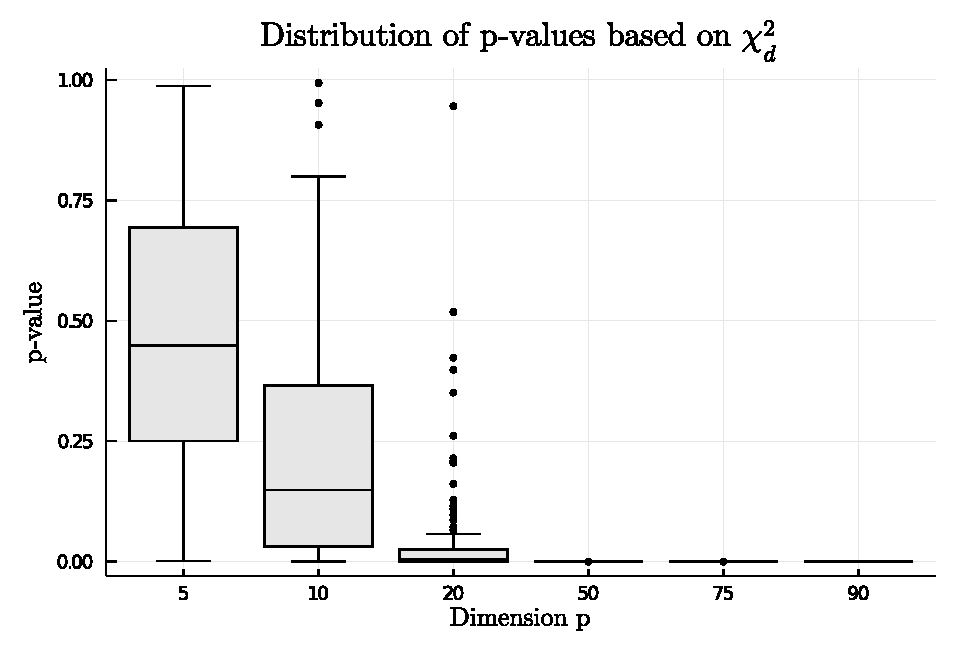
\includegraphics[width=7cm]{complete_to_chordless4cycle_chisq.eps}
    }
    \subfloat[\label{fig-size-4cycle-beta}]{
        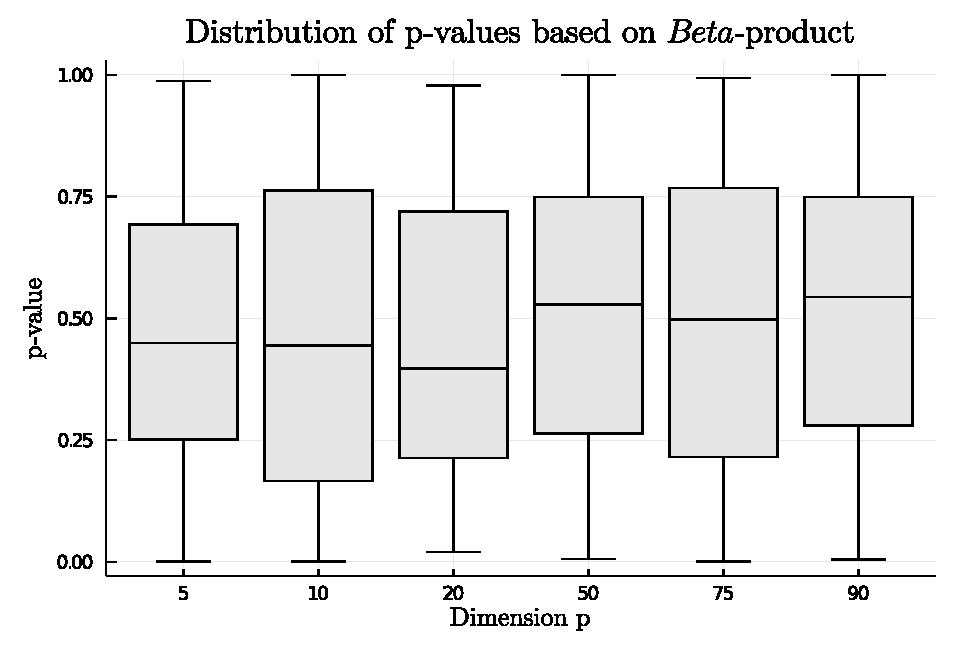
\includegraphics[width=7cm]{complete_to_chordless4cycle_beta.eps}
    }
\end{figure}

\cite{Tang2020}


\begin{figure}[!htbp]
    \centering
    \subfloat[\label{fig-power-4cycle-chisq}]{
        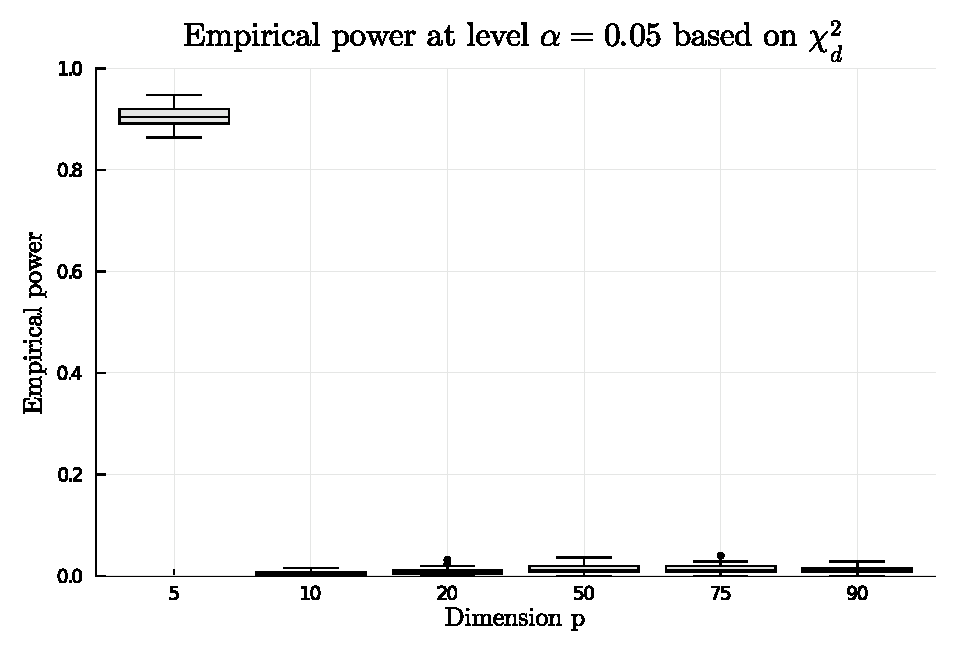
\includegraphics[width=7cm]{power_complete_to_chordless4cycle_chisq.eps}
    }
    \subfloat[\label{fig-power-4cycle-beta}]{
        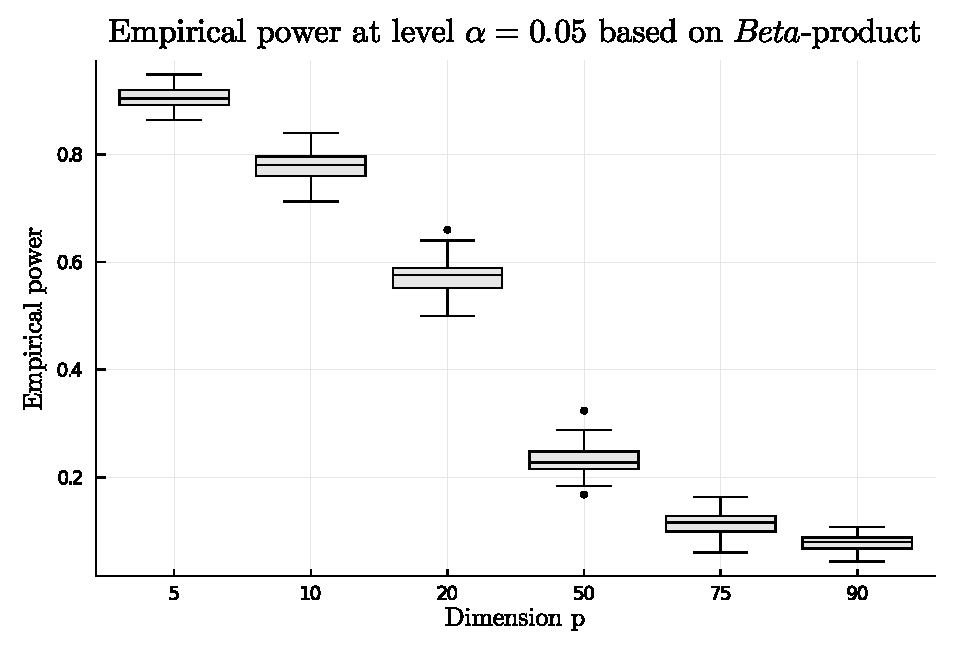
\includegraphics[width=7cm]{power_complete_to_chordless4cycle_beta.eps}
    }
\end{figure}

\begin{figure}[!htbp]
    \centering
    \subfloat[\label{fig-size-cycle-chisq}]{
        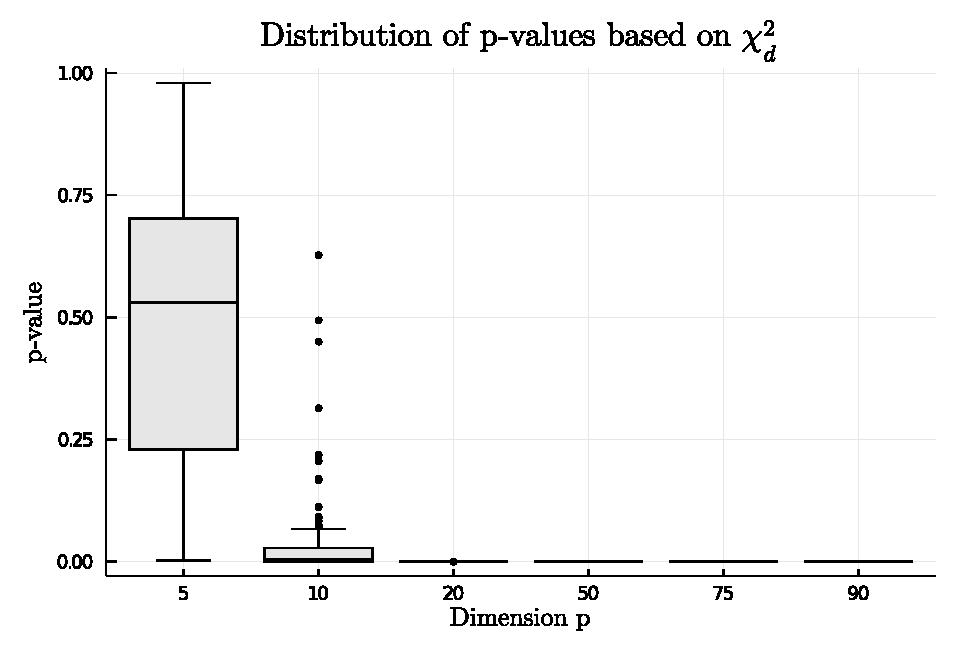
\includegraphics[width=7cm]{complete_to_pcycle_chisq.eps}
    }
    \subfloat[\label{fig-size-cycle-beta}]{
        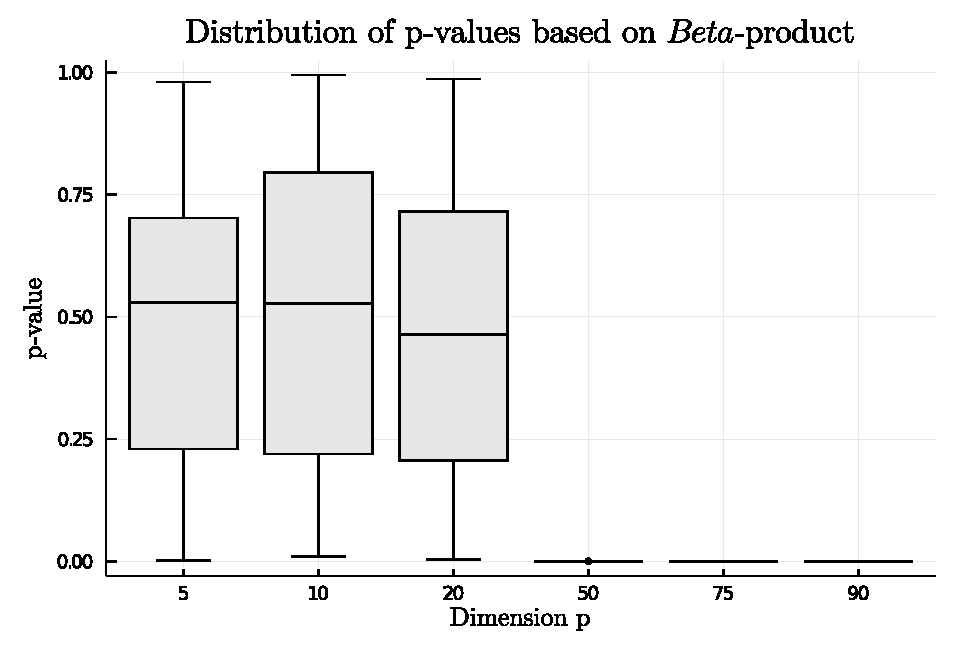
\includegraphics[width=7cm]{complete_to_pcycle_beta.eps}
    }
\end{figure}

\begin{figure}[!htbp]
    \centering
    \subfloat[\label{fig-power-cycle-chisq}]{
        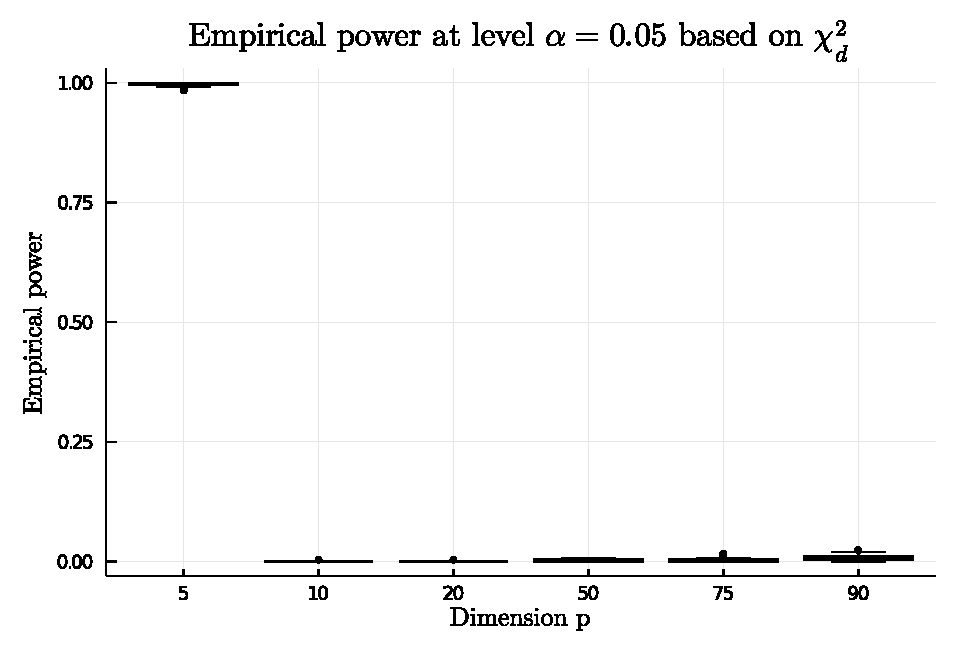
\includegraphics[width=7cm]{power_complete_to_cycle_chisq.eps}
    }
    \subfloat[\label{fig-power-cycle-beta}]{
        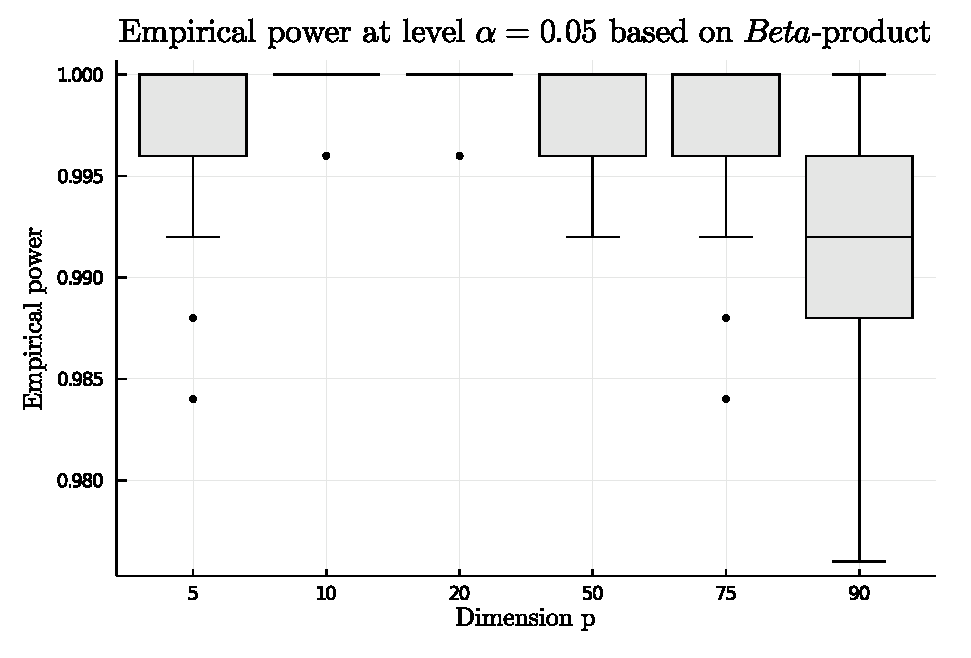
\includegraphics[width=7cm]{power_complete_to_cycle_beta.eps}
    }
\end{figure}


We now compare different properties of the hypothesis test based on the $\chi^2_d$ approximation to the likelihood ratio and the product of Beta distributions described in \note{todo ref}. We are interested in evaluating the size and power of the tests resulting from these two asymptotic approximations. The \textit{size} of a test is its probability of rejecting the null hypothesis when it is true, also called \textit{type I error}. The \textit{power} of a test is its probability to reject the null hypothesis when it is false. One is interested in tests maximizing power while keeping the probability of doing a type I error under a pre-defined level $\alpha$. In other words, a good test maximizes the probability of discovering true phenomena while keeping the probability of making a false discovery under control.

Evaluating the size of a test is equivalent to evaluating the quality of the asymptotic distribution approximation used by the test in finite sample. 


% \begin{figure}
%     \centering
%     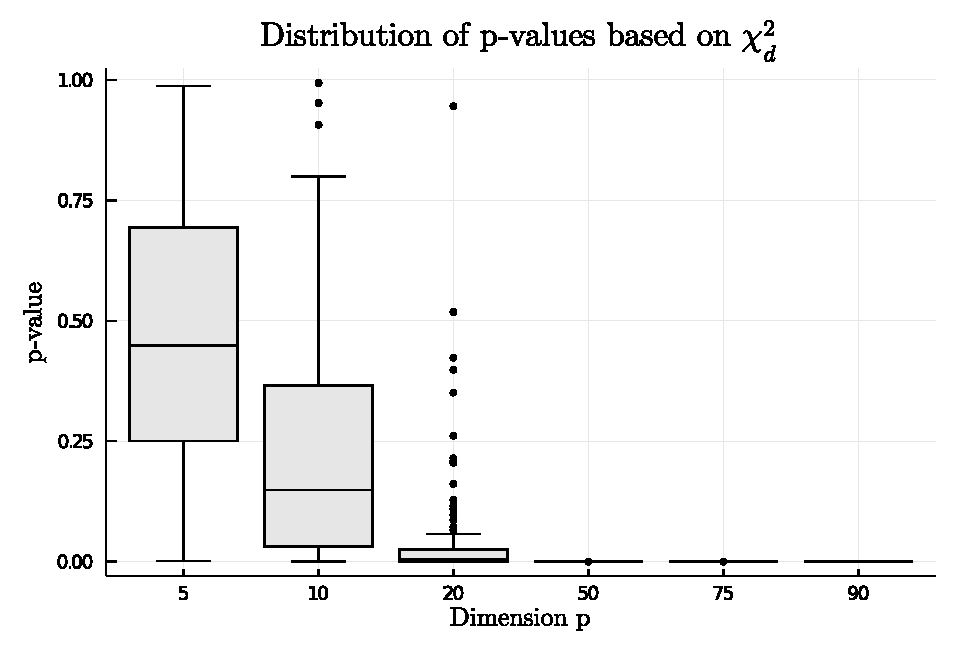
\includegraphics[width=7cm]{complete_to_chordless4cycle_chisq.eps}
% \end{figure}

